\documentclass[12pt]{scrartcl}


\setlength{\parindent}{0pt}
\setlength{\parskip}{.25cm}

\usepackage{graphicx}

\usepackage{xcolor}

\definecolor{darkred}{rgb}{0.5,0,0}
\definecolor{darkgreen}{rgb}{0,0.5,0}
\usepackage{hyperref}
\hypersetup{
  letterpaper,
  colorlinks,
  linkcolor=red,
  citecolor=darkgreen,
  menucolor=darkred,
  urlcolor=blue,
  pdfpagemode=none,
  pdftitle={CSCE 156 Lab Handout},
  pdfauthor={Christopher M. Bourke},
  pdfsubject={},
  pdfkeywords={}
}

\definecolor{MyDarkBlue}{rgb}{0,0.08,0.45}
\definecolor{MyDarkRed}{rgb}{0.45,0.08,0}
\definecolor{MyDarkGreen}{rgb}{0.08,0.45,0.08}

\definecolor{mintedBackground}{rgb}{0.95,0.95,0.95}
\definecolor{mintedInlineBackground}{rgb}{.90,.90,1}

%\usepackage{newfloat}
\usepackage[newfloat=true]{minted}
\setminted{mathescape,
               linenos,
               autogobble,
               frame=none,
               framesep=2mm,
               framerule=0.4pt,
               %label=foo,
               xleftmargin=2em,
               xrightmargin=0em,
               startinline=true,  %PHP only, allow it to omit the PHP Tags *** with this option, variables using dollar sign in comments are treated as latex math
               numbersep=10pt, %gap between line numbers and start of line
               style=default, %syntax highlighting style, default is "default"
               			    %gallery: http://help.farbox.com/pygments.html
			    	    %list available: pygmentize -L styles
               bgcolor=mintedBackground} %prevents breaking across pages
               
\setmintedinline{bgcolor={mintedBackground}}
\setminted[text]{bgcolor={mintedBackground},linenos=false,autogobble,xleftmargin=1em}
%\setminted[php]{bgcolor=mintedBackgroundPHP} %startinline=True}
\SetupFloatingEnvironment{listing}{name=Code Sample}
\SetupFloatingEnvironment{listing}{listname=List of Code Samples}


\usepackage{tikz}
\usetikzlibrary{calc,shapes.multipart,chains,arrows}

\title{CSCE 156 -- Computer Science II}
\subtitle{Lab 15.0 - Binary Search Trees}
\author{~}
\date{~}

\begin{document}

\maketitle

\section*{Prior to Lab}

\begin{enumerate}
  \item Review this laboratory handout prior to lab.
  \item Read and understand relevant materials on Binary 
    Search Trees and Heaps
\end{enumerate}

\section*{Lab Objectives \& Topics}
Following the lab, you should be able to:
\begin{itemize}
  \item Be familiar with Binary Search Trees and Heaps
  \item Be able to implement and utilize tree traversal algorithms
  \item Be able to utilize BSTs and Heaps in an application
\end{itemize}


\section*{Peer Programming Pair-Up}

To encourage collaboration and a team environment, labs will be
structured in a \emph{pair programming} setup.  At the start of
each lab, you will be randomly paired up with another student 
(conflicts such as absences will be dealt with by the lab instructor).
One of you will be designated the \emph{driver} and the other
the \emph{navigator}.  

The navigator will be responsible for reading the instructions and
telling the driver what to do next.  The driver will be in charge of the
keyboard and workstation.  Both driver and navigator are responsible
for suggesting fixes and solutions together.  Neither the navigator
nor the driver is ``in charge.''  Beyond your immediate pairing, you
are encouraged to help and interact and with other pairs in the lab.

Each week you should alternate: if you were a driver last week, 
be a navigator next, etc.  Resolve any issues (you were both drivers
last week) within your pair.  Ask the lab instructor to resolve issues
only when you cannot come to a consensus.  

Because of the peer programming setup of labs, it is absolutely 
essential that you complete any pre-lab activities and familiarize
yourself with the handouts prior to coming to lab.  Failure to do
so will negatively impact your ability to collaborate and work with 
others which may mean that you will not be able to complete the
lab.  

Clone the starter code for this lab from GitHub using the following
url: \url{https://github.com/cbourke/CSCE156-Lab15}.

\section*{Binary Search Trees}

A Binary Search Tree (BST) is a data structure such that elements 
are stored in tree nodes.  Each tree node has a reference 
to its parent, left child, and right child.  Each node in a BST also 
has a key associated with it.  The Binary Search Tree Property is 
such that:
\begin{enumerate}
  \item All keys in a node's left-subtree are less than that node's key
  \item All keys in a node's right-subtree are greater than that node's key
\end{enumerate}  
An example is presented in Figure \ref{figure:bst}.

\begin{figure}[h]
\centering
%\documentclass{article}
%\usepackage{fullpage}
%\usepackage{tikz}
%\begin{document}
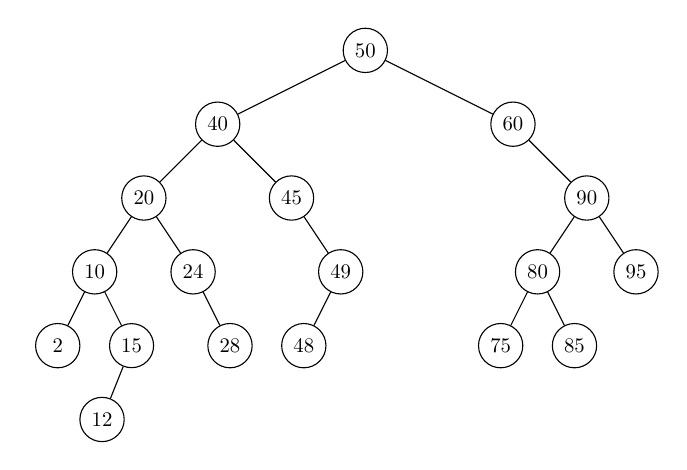
\begin{tikzpicture}[scale=0.75,transform shape,level distance=1.25cm,level/.style={sibling distance=5cm/#1},every node/.style={circle,draw,minimum size=.75cm}]
\node{$50$}
child {node {$40$} 
child {node {$20$} 
child {node {$10$} 
child {node {$2$} 
child[draw opacity=0.0] {}
child[draw opacity=0.0] {}
}
child {node[circle,draw,minimum size=.60cm] {$15$} 
child {node[circle,draw] {$12$}}
child[draw opacity=0.0] {}
}
}
child {node {$24$} 
child[draw opacity=0.0] {}
child {node {$28$} 
child[draw opacity=0.0] {}
child[draw opacity=0.0] {}
}
}
}
child {node {$45$} 
child[draw opacity=0.0] {}
child {node {$49$} 
child {node {$48$} 
child[draw opacity=0.0] {}
child[draw opacity=0.0] {}
}
child[draw opacity=0.0] {}
}
}
}
child {node {$60$} 
child[draw opacity=0.0] {}
child {node {$90$} 
child {node {$80$} 
child {node {$75$} 
child[draw opacity=0.0] {}
child[draw opacity=0.0] {}
}
child {node {$85$} 
child[draw opacity=0.0] {}
child[draw opacity=0.0] {}
}
}
child {node {$95$} 
}
}
}
;
\end{tikzpicture}

%\end{document}
\caption{A binary search tree with integer keys}
\label{figure:bst}
\end{figure}

The basic functionality such as adding elements, searching for elements, 
and removing elements can be achieved with a complexity proportional to 
the tree's depth.  Searching, for example, starts at the root.  If the 
node corresponds to the element we are searching for we are done.  
Otherwise, if the node has a key value less than the element we are 
searching for we traverse to its right child.  If the node has a key 
value greater than the element we are searching for we traverse to its 
left child and repeat until we have found the node or we reach the 
end of a tree without finding our element.

An incomplete binary search tree Java implementation has been provided 
for you.  It has some basic functionality already.  Your activities 
will include adding additional methods to perform a search, and to 
traverse the tree using several different traversal strategies and to 
count the number of leaves in the tree.

A node in a binary tree is called a leaf if it has no children.  Since 
the structure of a binary search tree is determined by the order 
elements are entered, there is no easily computable formula for the 
number of leaves.  Instead, a BST needs to be traversed and the leaves 
counted up.  

There are three traversal strategies that you will implement.  The 
implementation is up to you; you may find that a recursive strategy 
is the quickest to implement or you may find a stack data structure 
useful.  Each of these strategies begins at the root and visits a 
node and its children in different orders.

\begin{itemize}
  \item Preorder Traversal: processes the node, then visits the 
    nodes in the left-subtree then in the right-subtree 
  \item Inorder Traversal: visits the left-subtree first, then the node 
    itself, then the right-subtree
  \item Postorder Traversal: visits the left-subtree first, then the right-
    subtree, then the node itself
\end{itemize}

\subsection*{Instructions}

\begin{enumerate}
  \item Implement the search algorithm described above (the 
    \mintinline{java}{findElement()} method)
  \item Implement the three ordering methods as described above
  \item Implement the \mintinline{java}{getNumLeaves()} method 
  \item Use these methods to answer the questions on your worksheet 
\end{enumerate}

\section*{Heaps}
    
A heap is a data structure similar to a binary search tree in that 
it has a binary tree structure.  The primary difference is that the 
key for each node in the tree is larger than \emph{both} of its 
children. There is no restriction on the relation between the keys 
of child nodes.  Another condition of heaps is that they are full 
binary trees: each level of the tree, with the possible exception 
of the final row has every node present.  This property ensures that 
operations such as add and remove (from the top) can be performed 
with $O(\log(n))$ operations.

Implementing a heap can be done using a dynamic array--the random 
access ensures the optimal behavior of operations.  For this 
activity, we will not be building a heap from scratch; rather we 
will be taking advantage of the Java Collection library's 
\mintinline{java}{PriorityQueue} class.  This class uses a 
\mintinline{java}{Comparator} provided at instantiation to maintain 
the following guarantee: any dequeue operation (poll) will return 
the element with the ``highest'' priority (the greatest value 
according to the \mintinline{java}{Comparator}).  The corresponding 
enqueue operation (offer) inserts elements into the priority queue.

One application of heaps sorting, in particular the heap sort 
algorithm.  The basic idea is that elements are removed from a 
list one-by-one and are placed on a heap.  Then, elements are 
successively removed from the heap and placed back into the list.  
The heap property guarantees that the maximal (or minimal) element 
is removed each time, imposing an ordering.

\subsection*{Instructions}

\begin{enumerate}
  \item Implement the \mintinline{java}{Heap} class as specified; 
    each method should be implemented using methods of the 
    underlying \mintinline{java}{PriorityQueue} (this is an
    excellent example of composition at work).
  \item Use this implementation to implement the 
    \mintinline{java}{heapSort()} method in the 
    \mintinline{java}{HeapSort} class.  This class has a 
    \mintinline{java}{main()} method which you can use to test 
    your implementation.
\end{enumerate}
    
\section*{Submission}

We have included a test suite of unit tests written in JUnit 
(\url{https://junit.org/junit5/}) a popular unit testing framework for
Java.  Even though the test driver (in the \mintinline{text}{src/test}
source folder) has no main method, you can still run it in Eclipse and
get a report on how many of the tests passed, failed or resulted in 
an unexpected exception.  Be sure all of the unit tests pass before
submitting your source files through webhandin.  You can rerun this
test suite in the webgrader to ensure everything works.  

\section*{Advanced Activity (Optional)}

Another tree traversal strategy is a Breadth-First-Search (BFS) traversal 
strategy.  Starting at the root, nodes are visited level-by-level 
in a left-to-right order.  Design (or research) and implement a 
BFS strategy on your binary search tree.  Hint: look at the 
non-recursive traversal strategies used in some of the methods 
provided to you.  Think of a similar strategy using a different data 
structure.

\end{document}
